\section{AMSI (Antimalware Scan Interface)}

The Antimalware Scan Interface (AMSI) is a standardized interface which Windows applications can use to interact with the antimalware software in use.

The following diagram illustrates from a high level how it works. the important thing to take away from this is that applications can make use of the functions \verb+AmsiScanBuffer+ and \verb+AmsiScanString+ to scan input for malicious content.

\verb+AmsiScanString+ uses \verb+AmsiScanBuffer+ underneath.

The AMSI feature is integrated into these components of Windows 10:  User Account Control, or UAC, PowerShell, Windows Script Host, JavaScript and VBScript Office VBA macros

in powershell usually an error is triggered:
\begin{verbatim}
This scipt contins malicious contnt and has been ...
\end{verbatim}

\begin{figure}[!ht]
  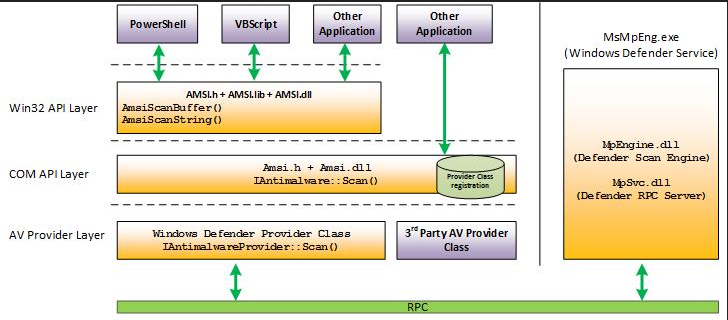
\includegraphics[width=\linewidth]{windows_knowledge/security/images/amsi.png}
  \caption{AMSI}
  \label{fig:amsi}
\end{figure}

Some quick facts about how AMSI works:
\begin{itemize}
    \item 
        AMSI protects PowerShell by loading AMSI’s DLL (amsi.dll) into the PowerShell’s memory space.
    \item 
        AMSI protection does not distinguish between a simple user with low privileges and a powerful user, such as an administrator.
    \item 
        AMSI scans the PowerShell console input by using Windows Defender (Or another AV program installed) to determine whether to block the payload operation or allow it to continue
\end{itemize}
